\chapter{The Return of WMAN}
\program{WMAN}

\section{Introduction}
\label{ch27-intro}%hyperlabel{ch27-intro}%

Before my recent delving into George's
 SETW\program{SETW}, his Easy PEasy\program{EasyPEasy}     utilities and my brief foray into pdf magazine production, I was walking
    through the various requirements of setting up a window definition using
    WMAN\program{WMAN}. This edition continues from where we left off but incorporates
    George's utilities into the examples. As George has made it easy to write
    Pointer Environment programs, I think we should make use of his hard work.
    Code reuse is all the rage!

However, before we start coding, we better take a moment to discuss
    Application Sub-{}Windows.

\section{Application Sub-{}Windows}
\label{ch27-appl-wins}%hyperlabel{ch27-appl-wins}%

There are a number of uses for application sub-{}windows, for the
    program's display or to hold a menu, correctly known as an
 \emph{application window menu}. An application window is a
    variable thing and as such, can be defined in a number of ways. Because of
    this, and because an application can have multiple application
    sub-{}windows, when defining our main window (or the variable parts of our
    main window) we don't have a pointer to an application window. Instead, we
    have a pointer to a list of pointers and each of these, in turn, points to
    an application window definition. The list is terminated by a zero
    word.

\begin{note}
George isn't fond of having an application window just for display purposes and points out that information windows are much, much simpler. He is, of course, correct!
\end{note}  

The following is the relevant extracts from a definition of a main
    window which contains information windows, loose items and a pair of
    application sub-{}windows.

\begin{lstlisting}[firstnumber=1,caption={Example Application Sub-Window List Definition}]
; Main window definition :
           ...
           dc.w  info_list-*       ; Pointer to information window list
           dc.w  loos_list-*       ; Pointer to list of loose items
           dc.w  appw_list-*       ; Pointer to list of app windows
           ...

; Application window list :
appw_list  dc.w  appw_0-*          ; Pointer to 1st sub-window defn
           dc.w  appw_1-*          ; Pointer to 2nd sub-window defn
           dc.w  0                 ; No more app sub-windows
\end{lstlisting}

The definition of an application sub-{}window is described
    below.

\begin{lstlisting}[firstnumber=last,caption={Example Application Sub-Window Definition}]
; Application sub-window definition :
appw_0     dc.w  192               ; Width in pixels (+ scaling)
           dc.w  119               ; Height in pixels (+ scaling)
           dc.w    4               ; X org relative to 0 in main window
           dc.w   18               ; Y org relative to 0 in main window
           dc.b  256               ; Bit 7 set = clear window
           dc.b    0               ; Shadow depth - must be 0!
           dc.w    1               ; Border width
           dc.w    0               ; Border colour
           dc.w    7               ; Paper colour
           dc.w    0               ; Pointer to pointer sprite, or 0
           dc.w    0               ; User defined setup routine, or 0
           dc.w    0               ; User defined drawing routine, or 0
           dc.w    ahit0-*         ; Hit routine
           dc.w    0               ; Sub-window control routine, or 0
           dc.w    0               ; Max X control sections (splits)
           dc.w    0               ; Max Y control sections (splits)
           dc.b    9               ; Selection key
           dc.b    0               ; Spare byte - must be 0
           ...
\end{lstlisting}

For our current needs, this definition allows us to have a simple
    application sub-{}window with no pan and scroll control bars and no menu.
    The user defined setup and drawing routines are most often defined as zero
    words to allow WMAN\program{WMAN} to do the hard work.

\section{Application Sub-{}Window Hit Routines}

The hit routine for an application sub-{}window is called from within
    the \pe{WM\_RPTR} call either when you HIT in the window, or when you press the
    selection key for that sub-{}window. Similar to loose item action routines
    previously discussed, if the code exits with D0 set to zero, the \pe{WM\_RPTR}
    call will resume again -{} in other words, control will not return to your
    own code just yet -{} unless the hit code sets any event bits in the event
    vector. This is slightly different from loose item action routines in this
    respect.

On entry to a sub-{}window hit routine various registers are set with
    specific parameters as defined in \tablename~\ref{tab:ApplicationSubWindowHitRoutineRegisters}


\begin{table}[htbp]
\centering
\begin{tabular}{l p{0.8\textwidth}}
\toprule
\textbf{Register} & \textbf{Description}  \\
\midrule
%
D1.L & High word = pointer X position. Low word = pointer Y position in \emph{absolute} screen coordinates. Ie, the pointer position within the \emph{entire screen} and \emph{not} within the program's window or the application sub-window itself.\\
D2.W & Selection keystroke letter, in its upper cased format, or 1 = Hit/SPACE or 2 = DO/ENTER. If D2 is -1, then the application sub-window was ``hit'' by an external keystroke. Zero indicates no key was pressed.\\
D4.B & An \emph{event number}. This can only be 0, pt\_\_do (16) or pt\_\_cancel (17) as all other events are handled by WMAN\program{WMAN}. If you have a loose item with ESC as the selection keystroke, then the loose item action routine will catch the ESC keystroke - the application sub-window hit routine will not see it if the ESC causes the program to exit.\\
A0.L & Channel id.\\
A1.L & Pointer to the status area.\\
A2.L & WMAN vector.\\
A3.L & Pointer to sub-window definition.\\
A4.L & Pointer to window working definition.\\
%
\bottomrule
\end{tabular}
\caption{Application Sub-Window Hit Routine - Registers}
\label{tab:ApplicationSubWindowHitRoutineRegisters}
\end{table}

 
Hit routines should exit with D1, D5 -{} D7, A0 and A4 preserved to
    the same value that they had on entry to the routine. D2, D4, A1 -{} A3, A5
    and A6 are undefined on exit (which means that they don't care what value
    they have.) The hit code must set the SR according to the value in D0 on
    exit.

D3, on return from a hit routine, should normally be returned as per
    its value on entry. It is not used by \pe{WM\_RPTR} however, it is used by
    \pe{WM\_RPTRT} (read pointer with return on timeout) from
 WMAN\program{WMAN} 1.5 onwards. Wm\_rptr ignores the upper
    word of D3. If your read pointer loop is using the \pe{WM\_RPTRT} vector
    instead, and you have changed the value of D3 within the hit code, you
    must clear the high word on exit.

It is important to note that WMAN\program{WMAN}  \emph{doesn't} set the event bits for you, it is up to the
    hit code to do that for you. For example, if someone HITs the application
    window then the hit routine will be called with D2 = 1 which is also the
    case also when someone DOes the application window but the pt\_\_do bit in
    the window byte of the event vector will \emph{not} be
    set.

On exit, if D0 is clear and the status (Z) bit is set, control will
    return to the \pe{WM\_RPTR} loop and not to your application's code. To return
    to your own code, the hit routine needs to set at least one event bit in
    the event vector.

If an error is detected within the hit code, then it should exit
    with the appropriate error code in D0 and the status register set
    accordingly.

\section{Example Application Window}
\label{ch27-example-appl-wins}%hyperlabel{ch27-example-appl-wins}%

As before, we now create a useful (!) demonstration program to show
    us the simplest use of an application sub window. The program will look
    like the following when completed and running:

\begin{figure}[h]
\center
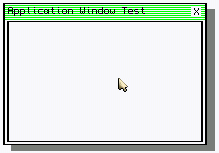
\includegraphics[width=0.5\textwidth]{Content/images/ApplTest_1.png}
\caption{Application Window Test}
\label{fig:ApplicationWindowTest}
\end{figure}

You can see from \figurename~\ref{fig:ApplicationWindowTest} how I'm sticking to accepted QDOSMSQ design     standards here can't you!

The window above consists of the following:
\begin{itemize}[itemsep=0pt]

\item{}An outline with white paper, a black single pixel border and a
        shadow. The default arrow sprite is used for the entire window.

\item{}A `caption bar' consisting of a single information window with
        green/white striped paper (paper colour 92).

\item{}Within the information window is a single information text
        object which is simply the program name.

\item{}Also located within the information window is one loose item
        containing a text object (`X') and this has the keypress code set up
        to close the window.

\item{}The remainder of the outline is filled with an application
        window, with white paper and a black single pixel border. (No shadow -{}
        they are forbidden for application windows!). This window also uses
        the default arrow sprite and has a selection key of TAB. This means
        that if you press the TAB key, the pointer will jump into the
        application sub-{}window.

\end{itemize}

The window was set up using SETW\program{SETW} as
    follows:
\begin{enumerate}
\item{When prompted for `name\$' enter
 \emph{ApplTestWin}.
}
\item{On the `Alter Text' screen.
\begin{itemize}[itemsep=0pt]

\item{}Press N for new, type `X' (without the quotes) then
            ENTER.

\item{}Press N for new, type `Application Window Test' (without the
            quotes) then ENTER

\item{}Press ESC.

\end{itemize}
}
\item{On the `Alter Sprite' screen.
\begin{itemize}[itemsep=0pt]

\item{}Press ESC.

\end{itemize}
}
\item{On the `Alter Blob' screen.
\begin{itemize}[itemsep=0pt]

\item{}Press ESC.

\end{itemize}
}
\item{On the `Alter Patt' screen.
\begin{itemize}[itemsep=0pt]

\item{}Press ESC.

\end{itemize}
}
\item{Number of main windows = 1
}
\item{Number of Loose Items = 1
}
\item{Number of Information windows = 1
}
\item{Number of IW Objects = 1
}
\item{Number of application windows = 1
}
\item{Application windows menu items = 0
}
\item{For main window 1:
\begin{itemize}[itemsep=0pt]

\item{}Shadow = 2

\item{}Border size = 1

\item{}Border colour = colour\_ql -{}>{} black

\item{}Paper colour -{} colour\_ql -{}>{} white

\item{}Sprite = arrow

\end{itemize}
}
\item{Loose Items:
\begin{itemize}[itemsep=0pt]

\item{}Press N for `system palette defaults'

\item{}Confirm N when prompted again for defaults

\item{}Border size = 1

\item{}Border colour = colour\_ql -{}>{} black

\item{}Unavailable background = colour\_ql -{}>{} white

\item{}Unavailable Ink = colour\_ql -{}>{} grey

\item{}Available background = colour\_ql -{}>{} white

\item{}Available Ink = colour\_ql -{}>{} black

\item{}Selected background = colour\_ql -{}>{} green

\item{}Selected Ink = colour\_ql -{}>{} black

\end{itemize}
}
\item{Loose Item 1:
\begin{itemize}[itemsep=0pt]

\item{}Type = text

\item{}Object -{}>{} select the `X' text object

\item{}Selection key = ESC

\end{itemize}
}
\item{Information Window 1:
\begin{itemize}[itemsep=0pt]

\item{}Border size = 0

\item{}Paper = colour\_ql -{}>{} No 92

\end{itemize}
}
\item{Object 1:
\begin{itemize}[itemsep=0pt]

\item{}Type = text

\item{}Object -{}>{} select the `Application Window Test' text
            object.

\item{}Colour = colour\_ql -{}>{} black

\item{}Xcsize = 0

\item{}Ycsize = 0

\end{itemize}
}
\item{Application Window 1:
\begin{itemize}[itemsep=0pt]

\item{}Border size = 1

\item{}Border colour = colour\_ql -{}>{} black

\item{}Paper colour = colour\_ql -{}>{} white

\item{}Sprite = arrow

\item{}Selection key = TAB

\end{itemize}
}
\item{Main window size: (Use the arrow keys to change the size, press
        ENTER when correct)
\begin{itemize}[itemsep=0pt]

\item{}Width = 200

\item{}Height = 140

\item{}Do you want a variable window = N

\item{}Set the origin to 0,0 (Press ENTER when correct)

\end{itemize}
}
\item{Loose Item 1: (Toggle hit/position with F2. Press ENTER when
        correct)
\begin{itemize}[itemsep=0pt]

\item{}Hit size = 10 x 10

\item{}Position = 186 x 3

\end{itemize}
}
\item{Information Window 1: (Toggle size/position with F2. Press ENTER
        when correct)
\begin{itemize}[itemsep=0pt]

\item{}Size = 200 x 16

\item{}Position = 0 x 0

\item{}Object position = 2 x 2

\end{itemize}
}
\item{Application Window 1: (Toggle size/position with F2. Press ENTER
        when correct)
\begin{itemize}[itemsep=0pt]

\item{}Size = 192 x 119

\item{}Position = 4 x 18

\end{itemize}
}
\end{enumerate}

When you have completed this procedure, and
 SETW\program{SETW} has exited, you should save the file
 ram1\_ApplTestWin\_asm to a safer place. The file
    should look like the following, although I have added some extra comments
    to my copy of the generated code.

\begin{lstlisting}[firstnumber=1,caption={Test Window - ApplTestWin\_asm}]
; ApplTestWin_asm

; Undefined Labels - need to be defined elsewhere in my own code.
;     ahit0   - application window 0 hit action routine.
;     afun0_0 - Loose item 0 hit action routine.

; Labels for External Use
;     wst0    - Window status area
;     wd0     - Window definition address
;     ww0_0   - Window default size
;     ww0_1   - Window button size

SYS_SPR  dc.w       0,1,2,3,4,5,6,7,8,9,10,11,12,13,14,15,16
         dc.w       17,18,19,20,21,22,23,24,25,26,27,28,29,30
         dc.w       31,32,33,34,35,36,37


; Definition of all text objects here

txt0     dc.w       txt0_e-2-txt0
         dc.b       "X"
txt0_e   ds.b       0
         ds.w       0

txt1     dc.w       txt1_e-2-txt1
         dc.b       "Application Window Test"
txt1_e   ds.b       0
         ds.w       0


; Application window list.
app_list0
         dc.w       appw0-*
         dc.w       0


; Application windows 0 definition.
appw0    dc.w       192       xsize
         dc.w       119       ysize
         dc.w       4         xorg
         dc.w       18        yorg
         dc.w       256       flag
         dc.w       1         borw
         dc.w       0         borc
         dc.w       7         papr
         dc.w       0         pspr *
         dc.w       0         setr *
         dc.w       0         draw *
         dc.w       ahit0-*   hit *
         dc.w       0         cntrl *
         dc.w       0         nxsc
         dc.w       0         nysc
         dc.b       9         skey
         dc.b       0         spr1

; Information Object(s)
pobl0    dc.w       138       xsize
         dc.w       10        ysize
         dc.w       2         xorg
         dc.w       2         yorg
         dc.b       0         type
         dc.b       0         spar
         dc.l       0         Ink, xcsize,ycsize
         dc.w       txt1-*    pobj *
         dc.w       -1

; Information window(s)
infw0    dc.w       200       xsize
         dc.w       16        ysize
         dc.w       0         xorg
         dc.w       0         yorg
         dc.w       0         flag
         dc.w       0         borw
         dc.w       526       borc
         dc.w       92        papr
         dc.w       pobl0-*   pobl *
         dc.w       -1        end

; Loose item(s)
litm0    dc.w       10,10     xsize, ysize
         dc.w       186,3     xorg, yorg
         dc.b       0,0       xjst, yjst
         dc.b       0,3       type, skey
         dc.w       txt0-*    pobj *
         dc.w       0         item
         dc.w       afun0_0-* pact *
         dc.w       -1        end

litm1    dc.w       16404,12  xsize, ysize
         dc.w       0,0       xorg, yorg
         dc.b       0,0       xjst, yjst
         dc.b       0,0       type, skey
         dc.w       0         pobj *
         dc.w       0         item
         dc.w       0         pact *
         dc.w       -1        end

; Window definition
wd0      dc.w       200       xsize
         dc.w       140       ysize
         dc.w       0         xorg
         dc.w       0         yorg
         dc.w       258       flag
         dc.w       1         borw
         dc.w       0         borc
         dc.w       7         papr
         dc.w       0         sprt *
         dc.w       1         curw
         dc.w       0         curc
         dc.w       7         uback
         dc.w       255       uink
         dc.w       0         ublob *
         dc.w       0         upatt *
         dc.w       7         aback
         dc.w       0         aink
         dc.w       0         ablob *
         dc.w       0         apatt *
         dc.w       4         sback
         dc.w       0         sink
         dc.w       0         sblob *
         dc.w       0         spatt *
         dc.w       0         help
         dc.w       200       xsize
         dc.w       140       ysize
         dc.w       infw0-*   pinfo *
         dc.w       litm0-*   plitem *
         dc.w       app_list0-*  pappl *
         dc.w       16384     xsize
         dc.w       12        ysize
         dc.w       0         pinfo *
         dc.w       litm1-*   plitem *
         dc.w       0         pappl *
         dc.w       -1

; Sizes
ww0_0    equ       290
ww0_1    equ       148

; Status Areas
wst0
         ds.b      65
wst0_e   ds.b      0
         ds.w      0
\end{lstlisting}

\section{Example Program}
\label{ch27-example-program}%hyperlabel{ch27-example-program}%

Having defined our application window test definition, we need a
    program to run it. However, we must also decide what the program is
    intended to do when running. As this is our first program with an
    application window, we will simply write some information to the
    application window when `things' happen.

I mentioned `code reuse' above, so the following is based very
    heavily on George's example code, with (I hope) all the unnecessary bits
    removed. Unnecessary, that is, for this example of mine!

The following is enough of a test harness to get our newly designed
    window up and running, but only the ESC key and the `X' loose item works.
    The rest of the program will come later.

In the source code that follows, where I use the `in' or the `lib'
    commands, you will need to replace `win1\_georgegwilt\_' with the location
    of the files being included. Unless you have exactly the same source setup
    as I do!

We start, as ever, with a standard QDOSMSQ job header and then pull
    in the various include files from Easy PEasy\program{EasyPEasy}. Three offsets into the job's
    data area are then defined.

\begin{lstlisting}[firstnumber=1,caption={ApplTest\_asm - Standard Job Header \& Equates}]
        bra.s start
        dc.l  0
        dc.w  $4afb

fname   dc.w  fname_e-fname-2
        dc.b  "Application Window Test 1"
fname_e ds.b  0
        ds.w  0

; We need the various equates files etc.

        in win1_georgegwilt_peass_keys_pe
        in win1_georgegwilt_peass_qdos_pt
        in win1_georgegwilt_peass_keys_wwork
        in win1_georgegwilt_peass_keys_wstatus
        in win1_georgegwilt_peass_keys_wman
        in win1_georgegwilt_peass_keys_wdef

id      equ 0                   ; Channel id storage
wmvec   equ 4                   ; WMAN vector storage
slimit  equ 8                   ; IOP_FLIM results - 4 words ...
;                               ; X-size, Y-size, X-org, Y-org
\end{lstlisting}

Following on from the above, we have the job's start and
    initialisation code. As the vast majority of this has been explained
    before in the introductory article on George's Easy
    PEasy\program{EasyPEasy}, I shall not go into it again here. See \emph{Easy
    PEasy Part 1} in \emph{Volume 14 Issue 3} for full
    details.

\begin{lstlisting}[firstnumber=last,caption={ApplTest\_asm - Initialisation}]
start   lea (a6,a4.l),a6        ; Make A6 point to the job's dataspace
        bsr op_con              ; Open a con channel
        move.l a0,id(a6)        ; And store the channel id
        moveq #iop_pinf,d0      ; Trap to get Pointer Information
        moveq #-1,d3            ; Timeout
        trap #3                 ; Do it
        tst.l d0                ; Is ptr_gen present?
        bne sui                 ; No, bale out via SUI
        move.l a1,wmvec(a6)     ; Yes, store the WMAN vector
        beq sui                 ; Oops! WMAN wasn't actually found

flim    movea.l a1,a2           ; The WMAN vector is required in A2
;                               ; The channel id is already in A0
        lea slimit(a6),a1       ; Result buffer
        moveq #iop_flim,d0      ; Query maximum size of window
        moveq #0,d2             ; D2 must be zero
;                               ; D3 is preserved timeout from above
        trap #3                 ; Do it (No errors)
        tst.l d0                ; Did it work?
        bne sui                 ; No, exit via SUI

        subi.l #$C0008,(a1)     ; Adjust max height & width for shadow
;                               ; and borders. 
        lea wd0,a3              ; Get address of window definition
        move.l #ww0_0,d1        ; Get size of the working definition
        bsr getsp               ; ALCHP memory and set A0 to address
        movea.l a0,a4           ; Which we save in A4
\end{lstlisting}

So far so good. Next we use a generic piece of code to go through
    the status area and set all the lose item status bytes to
    `available'.

\begin{lstlisting}[firstnumber=last,caption={ApplTest\_asm - Loose Item Initialisation}]
        lea wst0,a1             ; Status area starts here
        movea.l a1,a0           ; Copy to A0
        moveq #wst0_e-wst0-1,d1 ; How many bytes to clear - 1

st_clr  clr.b (a0)+             ; Clear one byte
        dbf d1,st_clr           ; Then the remainder
\end{lstlisting}

At this point we are just about ready to go. So, the next piece of
    code will call out the various WMAN\program{WMAN} routines to
    setup the window definition, position it on screen where the pointer
    currently is located and draw it before vanishing into the twilight zone
    that is the read pointer loop within WMAN\program{WMAN}. All
    of these have been described before so I don't go into detail.

\begin{lstlisting}[firstnumber=last,caption={ApplTest\_asm - Window Creation \& Display}]
        movea.l id(a6),a0       ; Get the channel id where we need it
;                                 A1 is the status area address
;                                 A3 is the window definition address
;                                 A4 is the working definition address
        move.l wd_xmin+wd_rbase(a3),d1 ; Get the minimum dimensions
        andi.l #$FFF0FFF,d1     ; Mask off any scaling factors
        jsr wm_setup(a2)        ; Set up the working definition

        moveq #-1,d1            ; Draw the window where the pointer is
        jsr wm_prpos(a2)        ; Position it as a primary window
        jsr wm_wdraw(a2)        ; Draw the contents
wrpt    jsr wm_rptr(a2)         ; Enter the "read pointer" loop in WMAN
\end{lstlisting}

At this point, WMAN\program{WMAN} takes over and we
    never get beyond the above code unless an event is detected -{} or set in an
    action routine -{} or an action routine flags an error. You will learn more
    about this as we add some meat to this programs workings later on.

The following code will exit from the program if an error occurred.
    The Z flag is already set or unset according to the value in D0.

\begin{note}
Of course, the following checks only work if the application sub-window hit routine, or the various loose item action routines set D4 first, then D0. Otherwise, we need to make sure that the Z flag is set according to D0 before we test it.
\end{note}

\begin{lstlisting}[firstnumber=last,caption={ApplTest\_asm - Error Handling},label={lst:ApplTestErrorHandling}]
        beq.s no_err            ; Since D0 is zero D4 is non zero
        bra sui                 ; An error occurred exit via SUI
\end{lstlisting}

If we are here, we need to check for any events that may have been
    detected or set in an action routine. In this example, we don't check
    every event, only the CANCEL event caused by the ESC key being
    pressed.

On return from the \pe{WM\_RPTR} call, A0 is the channel id and A4 is the
    working definition address.

\begin{lstlisting}[firstnumber=last,caption={ApplTest\_asm - Event Handling}]
no_err  movea.l (a4),a1         ; Status area address
        btst #pt__can,wsp_weve(a1) ; Check for CANCEL event
        bne sui                 ; Exit

        bra.s wrpt              ; No more events, read pointer again
\end{lstlisting}

As mentioned above, this example currently is only checking for the
    ESC key being pressed. However, we have a loose item that can also be
    clicked to escape from the program. Rather than handling the ESC key and
    the loose item separately, we simply set the CANCEL event within the loose
    item action routine and let WMAN\program{WMAN} take care of
    it by passing control out of the read pointer loop into the above event
    handling code.

The following is the loose item action routine to do this.

\begin{lstlisting}[firstnumber=last,caption={ApplTest\_asm - ESC Loose Item Action Routine}]
; Loose item action routine

afun0_0 bset  #pt__can,wsp_weve(a1) ; Set the CANCEL event bit
        moveq #pt__can,d4         ; CANCEL event number
        moveq #0,d0               ; No errors
        rts                       ; Exit here and exit from wm_rptr too
\end{lstlisting}

Because we have an application window defined, then the following is
    the default application window hit routine. When you hit the application
    window, or press the TAB key, the following code is executed. The default
    simply sets the registers to show no errors, no events and returns control
    back to the \pe{WM\_RPTR} loop.

\begin{lstlisting}[firstnumber=last,caption={ApplTest\_asm - Application Window HIT Routine}]
; Application sub-window hit routine

ahit0   moveq #0,d4
        moveq #0,d0
        rts
\end{lstlisting}

\begin{note}
The loose item action routine and application window hit routine
      names, \texttt{afun0\_0} and \texttt{ahit0} are hard coded by
 SETW\program{SETW} and, unless we physically edit the code
      generated by SETW\program{SETW}, we must use the names
 SETW\program{SETW} chooses for us.

There is a pattern to the names though, \texttt{ahit0} is the application
      sub-{}window hit routine for application sub-{}window zero. \texttt{Ahit1} would be
      the hit routine for sub-{}window 1 and so on. For loose items, you have a
      layout number and a loose item number to contend with. So \texttt{afun0\_0} is for
      layout zero and loose item zero within that layout. \texttt{Afun0\_1} is the next
      loose item within that layout, and so on.

Note also, if, as above, the hit routine sets D4 first, then D0 prior to exiting, the code that checks for errors need not execute an instruction to set the Z flag according to D0, it can simply test the Z flag immediately. See line 68 in \lstlistingname~\ref{lst:ApplTestErrorHandling} above.
\end{note}

The remainder of the code, so far, consists of helper routines and
    is shown below without any further discussion.

\begin{lstlisting}[firstnumber=last,caption={ApplTest\_asm - Console Handling}]
; Various helper routines go here...

con     dc.w con_e-con-2          ; Size of channel definition
        dc.b 'con'
con_e   equ *

op_con  lea  con,a0               ; We want a console
        moveq #-1,d1              ; For this job
        moveq #0,d3               ; Open type = "OPEN"
        moveq #io_open,d0
        trap #2                   ; Do it
        rts
\end{lstlisting}

And finally, we need to load in the window definition we generated
    using SETW\program{SETW} and all the Easy
    PEasy\program{EasyPEasy} code libraries supplied by George.

\begin{lstlisting}[firstnumber=last,caption={ApplTest\_asm - Incorporating the EasyPEasy Library}]
; Pull in our window definition file.

        in  win1_source_ApplTestWin_asm

; We need George's Easy PEasy code next.

        in  win1_georgegwilt_peass_peas_sym_lst
        lib win1_georgegwilt_peass_peas_bin

; And finally, George's sprites.

        in  win1_georgegwilt_peass_csprc_sym_lst
        lib win1_georgegwilt_peass_csprc_bin
\end{lstlisting}

Save the code as ApplTest\_asm. At least, that's
    what I called mine!

The code above can be assembled and executed and the window we
    designed a couple of issues ago will be displayed on screen. Currently it
    does nothing useful but if you press the TAB key when the pointer is
    outside the application window (but inside the main window) then you will
    see it jump into the application window. HITting the `X' loose item will
    cause the program to exit as will pressing the ESC key.

\section{Coming Up...}
\label{ch27-the-end}%hyperlabel{ch27-the-end}%

In the coming chapter we will add some code to this example to allow us to
    monitor events.

